
\chapter{Multidimensional Visual Analysis Tools}

\label{chap:MVATools}

MVA software is a type of computer program that is designed to help
analysts visualize and analyze complex data sets. These programs typically
include a wide range of tools and features that allow users to create and
manipulate graphical representations of the data, such as scatter plots,
parallel coordinates, and heat maps. By using these tools, analysts can
quickly and easily explore the data and gain insights that might not be
immediately apparent from looking at the raw data. MVA software is
commonly used in fields such as business, finance, and marketing to help
make data-driven decisions and uncover hidden trends in the data. In this
section, we will review some popular MVA software programs.




\section{InfoScope}

InfoScope \parencite{InfoScope} is an interactive visualization tool
to access, explore, and communicate large or complex
datasets. InfoScope is available as free software with the last update
issued on \yearmonthday{2007}{2}{9}. InfoScope is available for Windows, 
macOS, and Linux.

InfoScope can visualize a collection of selected publicly available
datasets, mainly from the finance sector. InfoScope provides an overview
of global relationships between objects by using multiple views to show
different aspects of the data at the same time. InfoScope provides the
following views: \emph{Carto Plot}, \emph{Similarity Map} as
high-dimensional projections, \emph{Parallel Coordinates}, and \emph{Table
View}. InfoScope supports brushing and linking, so all views are highly
interactive and tightly linked. Specific numeric values of attributes can
be obtained by probing the objects in the views, and dynamic queries on a
combination of attributes can be executed using range sliders. All actions
are accompanied by visual feedback within a common frame of reference. The
visual representations make it easy to identify outliers, patterns, or
anomalies. InfoScope supports manual grouping of data by color.
Figure~\ref{fig:ScreenshotInfoScope} shows a screenshot of the InfoScope
tool.




\begin{figure}[tp]
\centering
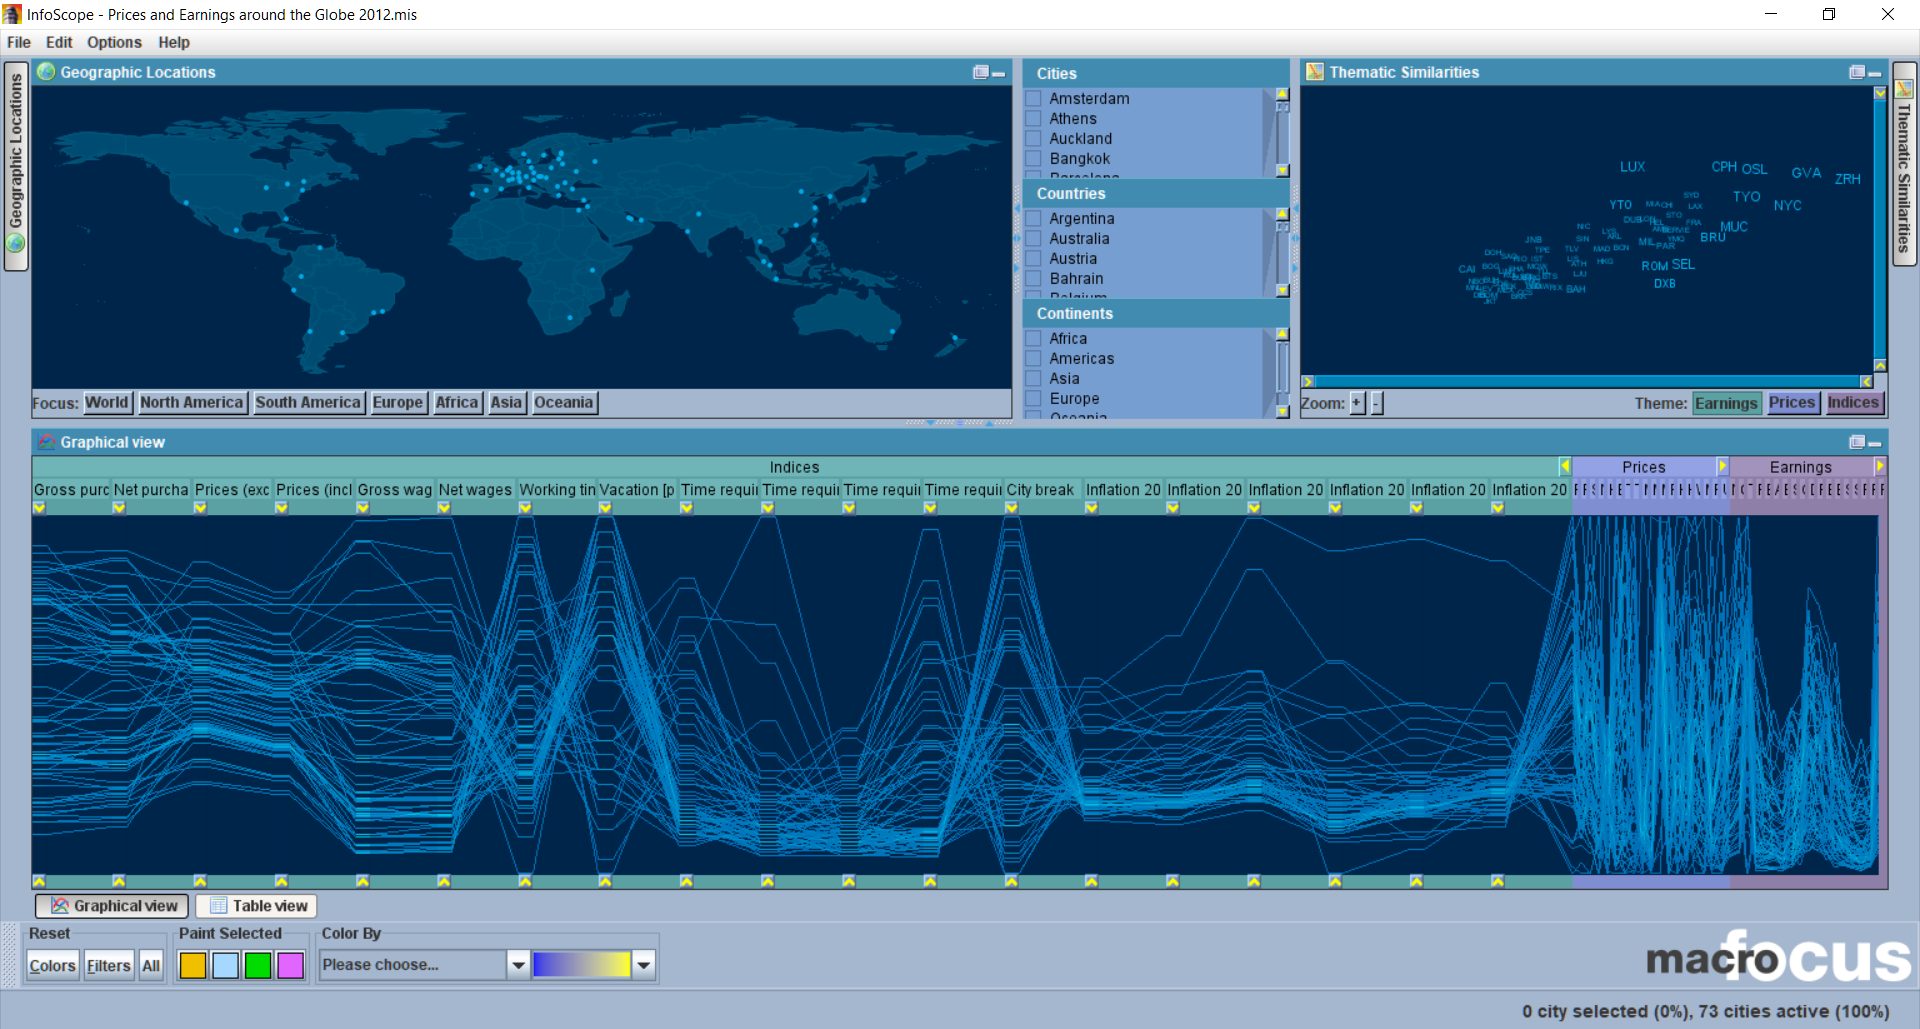
\includegraphics[keepaspectratio,width=\linewidth,height=\halfh]
{images/screenshot-infoscope.png}

\caption[InfoScope Dashboard]
{%
InfoScope dashboard displaying the \emph{Prices and Earnings around the Globe 2012} dataset.
}
\label{fig:ScreenshotInfoScope}
\end{figure}




\section{High-D}

High-D \parencite{HighD} is the successor to InfoScope. It offers similar
functionality with some improvements and added views. High-D is a
versatile tool for revealing hidden features, highlighting trends and
relationships, and finding anomalies in datasets of any size. At its heart
is a powerful interactive parallel coordinates plot for quick data access,
analytical, and presentation purpose. High-D is available as paid software
for 199 USD and with 30-day free evaluation period. The last update was
issued on \yearmonthday{2022}{12}{5}. High-D is available for Windows,
macOS, and Linux.


High-D can visualize a collection of selected publicly available datasets
as well as custom datasets. High-D provides an overview of global
relationships between objects by using multiple views to show different
aspects of the data at the same time. High-D provides the following views:
\emph{Parallel Coordinates}, \emph{Table Plot}, \emph{Distributions},
\emph{Scatter Plot Matrix}, \emph{Parallel Coordinates Matrix},
\emph{Scatter Plot}, \emph{Similarity Map} as high dimensional projections
(Sammon, Spring, t-SNE, and PCA), \emph{Tree Map}, and \emph{Carto Plot}.
High-D also manual grouping of data by color and automated clustering with
k-means++ algorithm. High-D supports brushing and linking, so all views
are highly interactive and tightly linked. It is possible to obtain
specific numeric values of attributes by examining the objects within the
views, and dynamic queries on a combination of attributes can be performed
using range sliders. All actions are accompanied by visual feedback within
a common frame of reference. The visual representations make it easy to
spot unusual data points, patterns, or anomalies.
Figure~\ref{fig:ScreenshotHighD} shows a screenshot of the High-D tool.




\begin{figure}[tp]
\centering
\includegraphics[keepaspectratio,width=\linewidth,height=\halfh]
{images/screenshot-highd.png}

\caption[High-D Dashboard]
{%
High-D dashboard displaying the \emph{Premier League Player Stats} dataset.
}
\label{fig:ScreenshotHighD}
\end{figure}




\section{GGobi}

GGobi \parencite{cook2007interactive} is a visualization program for
exploring high-dimensional data. GGobi is written in C and is available as
a free and open-source software with the last update issued on
\yearmonthday{2012}{6}{10}. GGobi is available for Windows, Apple macOS,
and Linux.

GGobi can visualize custom datasets and provides a dynamic and interactive
graphics as tours, where data is displayed in an animation. The data is
also available in the following views: \emph{Scatter Plot}, \emph{Scatter
Plot Matrix}, \emph{Parallel Coordinates}, \emph{Time Series},
\emph{Distributions} as bar charts. GGobi supports limited brushing. Views
offer limited interactivity and interpretability and are not closely
connected. Figure~\ref{fig:ScreenshotGGobi} shows a screenshot of the
GGobi tool.




\begin{figure}[tp]
\centering
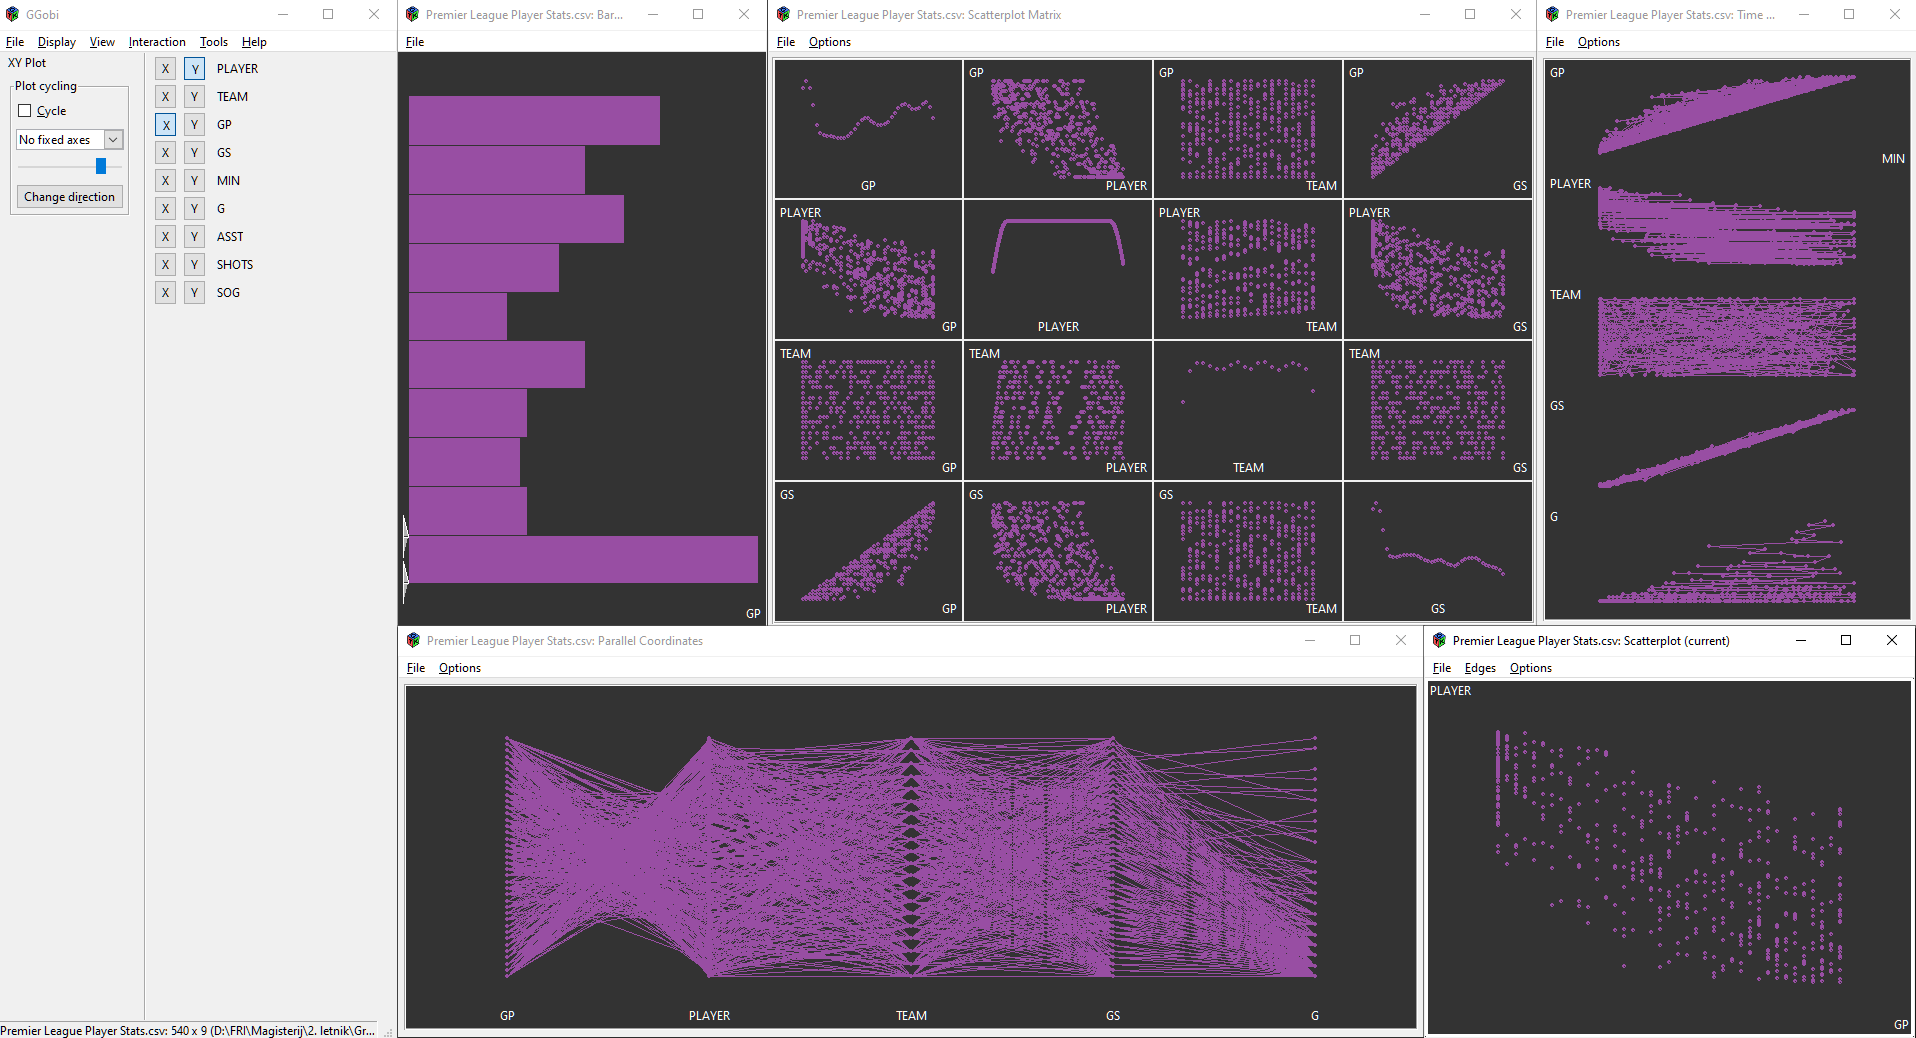
\includegraphics[keepaspectratio,width=\linewidth,height=\halfh]
{images/screenshot-ggobi.png}

\caption[GGobi Dashboard]
{%
GGobi dashboard displaying the \emph{Premier League Player Stats} dataset.
}
\label{fig:ScreenshotGGobi}
\end{figure}


\section{mVis}

mVis \parencite{CHEGINI20199} is a visual analytics tool for visualizing
multi-dimensional data. mVis is written in Java and is available as a free
and open-source software with the last update issued on
\yearmonthday{2021}{1}{20}. mVis is available for Windows, macOS, and
Linux.

mVis can visualize custom datasets and provides an overview of global
relationships between objects by using multiple views to show different
aspects of the data at the same time. mVis consists of four data
visualization views: \emph{Scatter Plot Matrix}, \emph{Scatter Plot},
\emph{Similarity Map} as high dimensional projections (t-SNE, PCA, and
MDS), and \emph{Parallel Coordinates}. mVis also consists of a panel for
controlling data partitions. All of the visualizations are interconnected
through standard brushing and linking, so that any changes or selections
made in one view are reflected in all of the other views. Additionally,
the user has the ability to close, rearrange, or expand any view as
needed.

mVis also supports creating and modifying ML models, specifically
introducing an interactive visual labeling technique that allows an
analyst to build and iteratively improve a ML classification model for
multi-dimensional data sets. This technique combines linked
visualizations, clustering, and active learning to allow the analyst to
interactively label a multi-dimensional dataset in an efficient manner.
Figure~\ref{fig:ScreenshotMVis} shows a screenshot of the mVis tool.




\begin{figure}[tp]
\centering
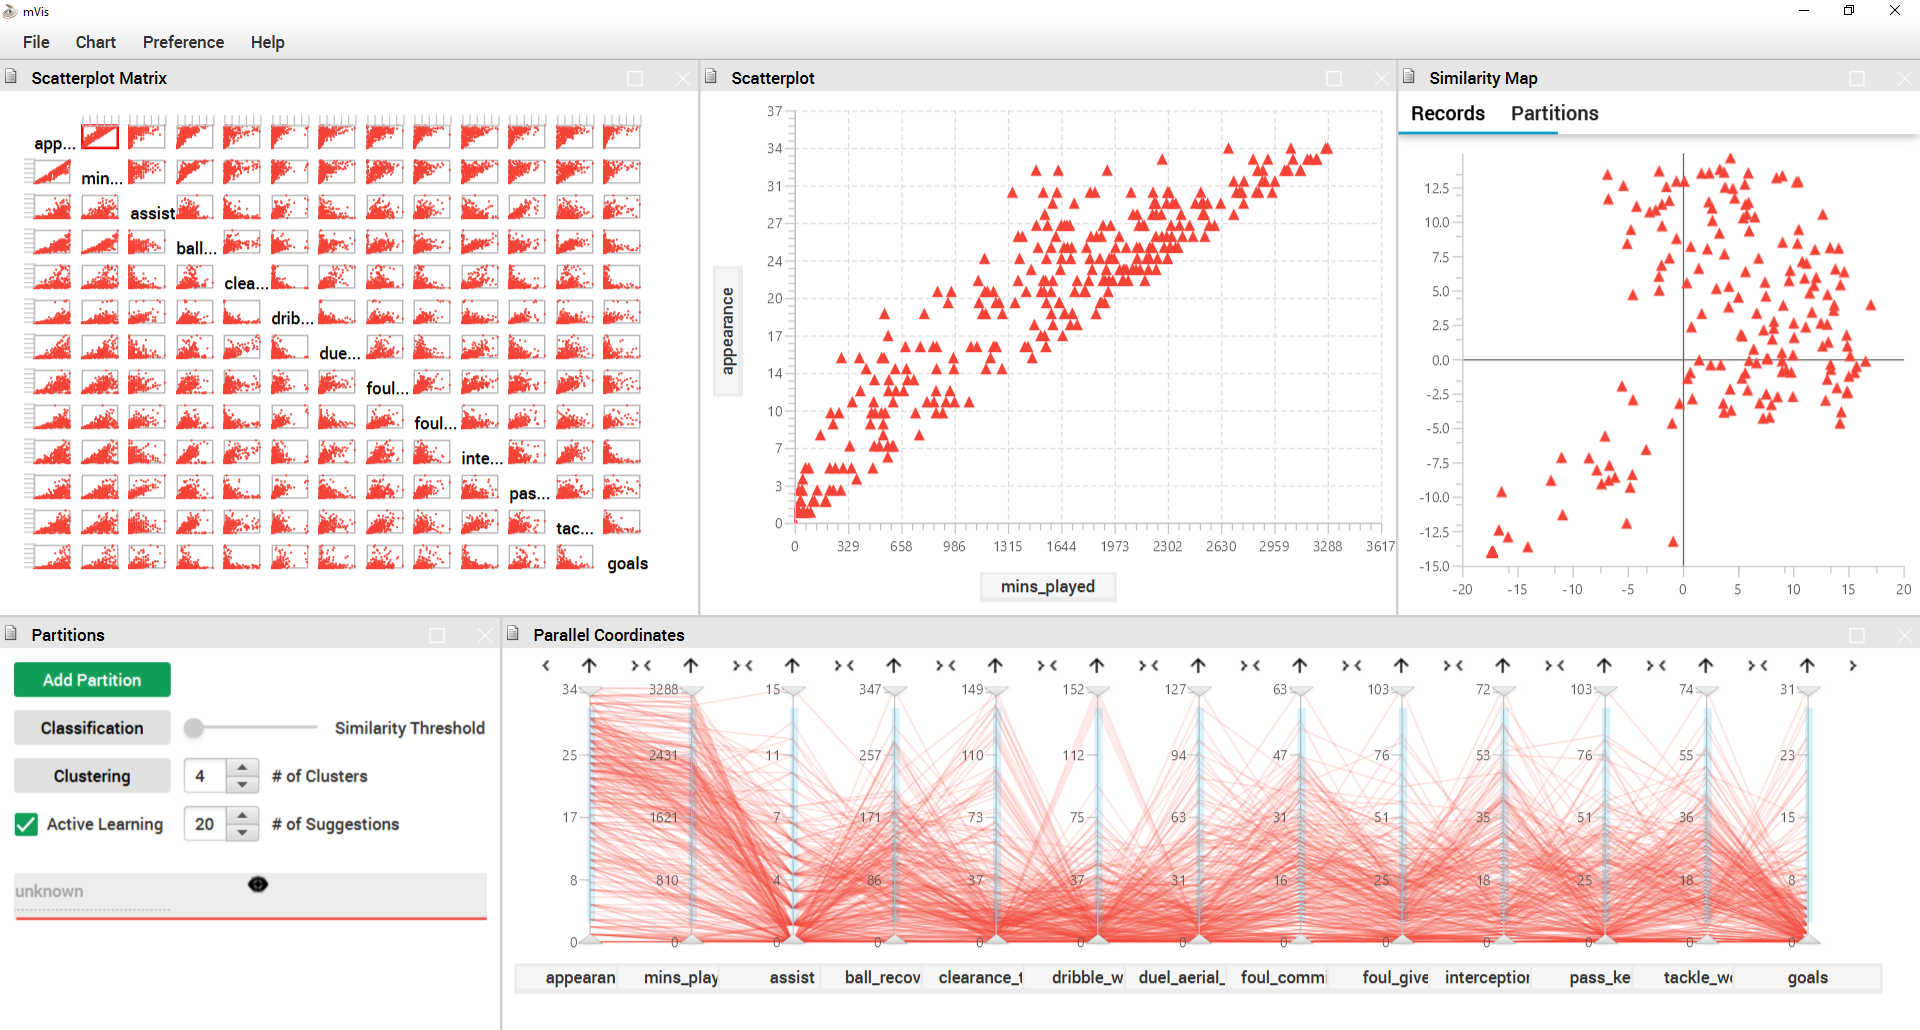
\includegraphics[keepaspectratio,width=\linewidth,height=\halfh,frame]
{images/screenshot-mvis.png}

\caption[mVis Dashboard]
{%
mVis dashboard displaying the \emph{mVis Custom Football Players} dataset.
}
\label{fig:ScreenshotMVis}
\end{figure}



\section{Improvise}

Improvise \parencite{Improvise} is a program that allows users to create
and interact with visualizations that are linked together in various ways.
Improvise is written in Java and is available as a free and open-source
software with the last update issued on \yearmonthday{2020}{10}{28}.
Improvise is available for Windows, macOS, and Linux.

The program uses a shared-object coordination model and a declarative
visual query language to give users control over how data is displayed in
multiple views. This allows users to create visualizations with a variety
of coordination patterns, such as synchronized scrolling, overview and
detail, drill-down, and semantic zoom. Improvise also has a user interface
that allows users to build and explore visualizations in a live
environment, making it easy to modify visualizations as needed. The goal
of Improvise is to provide a high level of coordination flexibility while
also being easy to use. It is designed to make it simple to create basic
coordination patterns and also possible to create more complex ones.
Figure~\ref{fig:ScreenshotImprovise} shows a screenshot of the Improvise
tool.




\begin{figure}[tp]
\centering
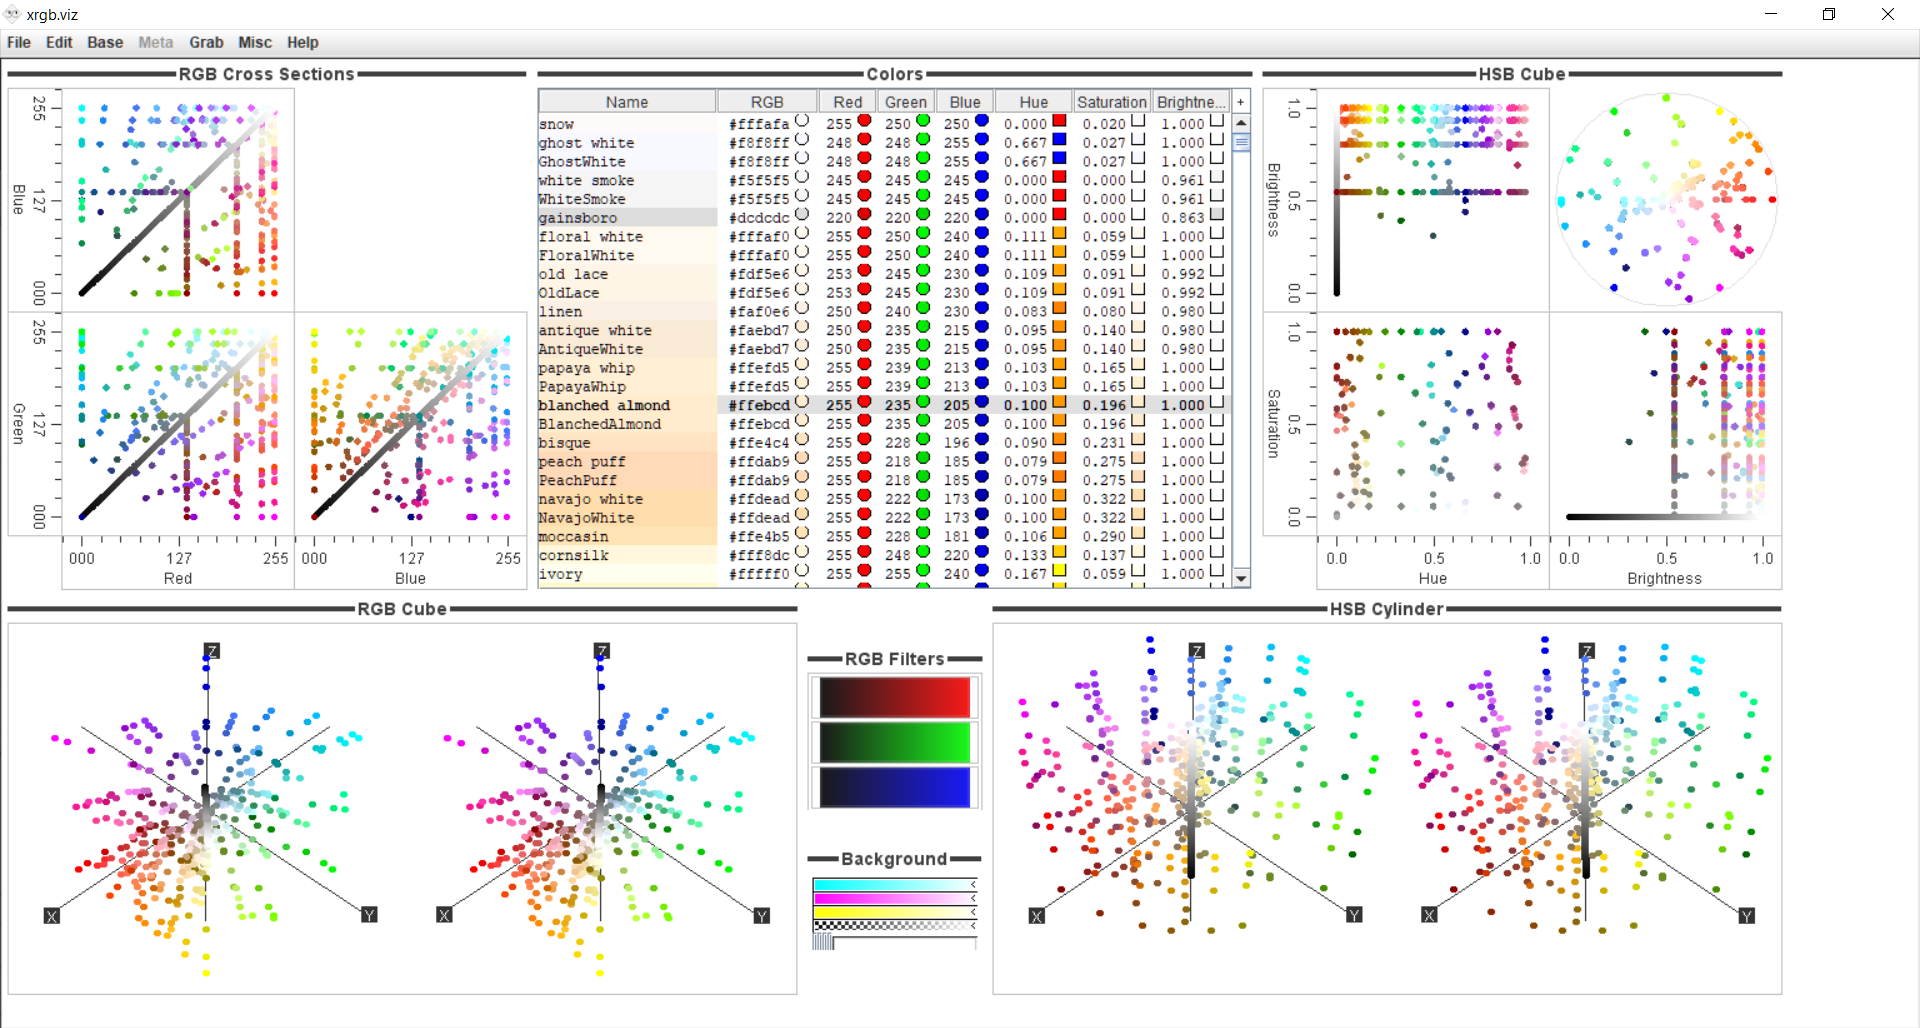
\includegraphics[keepaspectratio,width=\linewidth,height=\halfh, frame]
{images/screenshot-improvise.png}

\caption[Improvise Dashboard]
{%
Improvise dashboard displaying the \emph{Improvise Custom XRGB} dataset.
}
\label{fig:ScreenshotImprovise}
\end{figure}




\section{MyBrush}

MyBrush \parencite{koytek2017mybrush} is an application that allows users
to customize and control the brushing and linking process in their
visualizations. It provides flexibility by allowing users to specify the
source, link, and target of multiple brushes, and supports a variety of
visualization types and multiple simultaneous brushes. Improvise is
written in JavaScript and is available as a free and open-source web
application with the last update issued on \yearmonthday{2017}{9}{22}.

MyBrush serves as experimental software and offers limited functionality.
Its purpose is to explore the implemented brushing and linking
functionality.  A user can explore a predetermined set of data with the
following views: \emph{Scatter Plot}, \emph{Parallel Coordinates}, and
\emph{Bar Plot}. Any changes or selections made in one of the
visualizations will be reflected in all of the other views because they
are all interconnected through standard brushing and linking.
Figure~\ref{fig:ScreenshotMyBrush} shows a screenshot of the MyBrush tool.




\begin{figure}[tp]
\centering
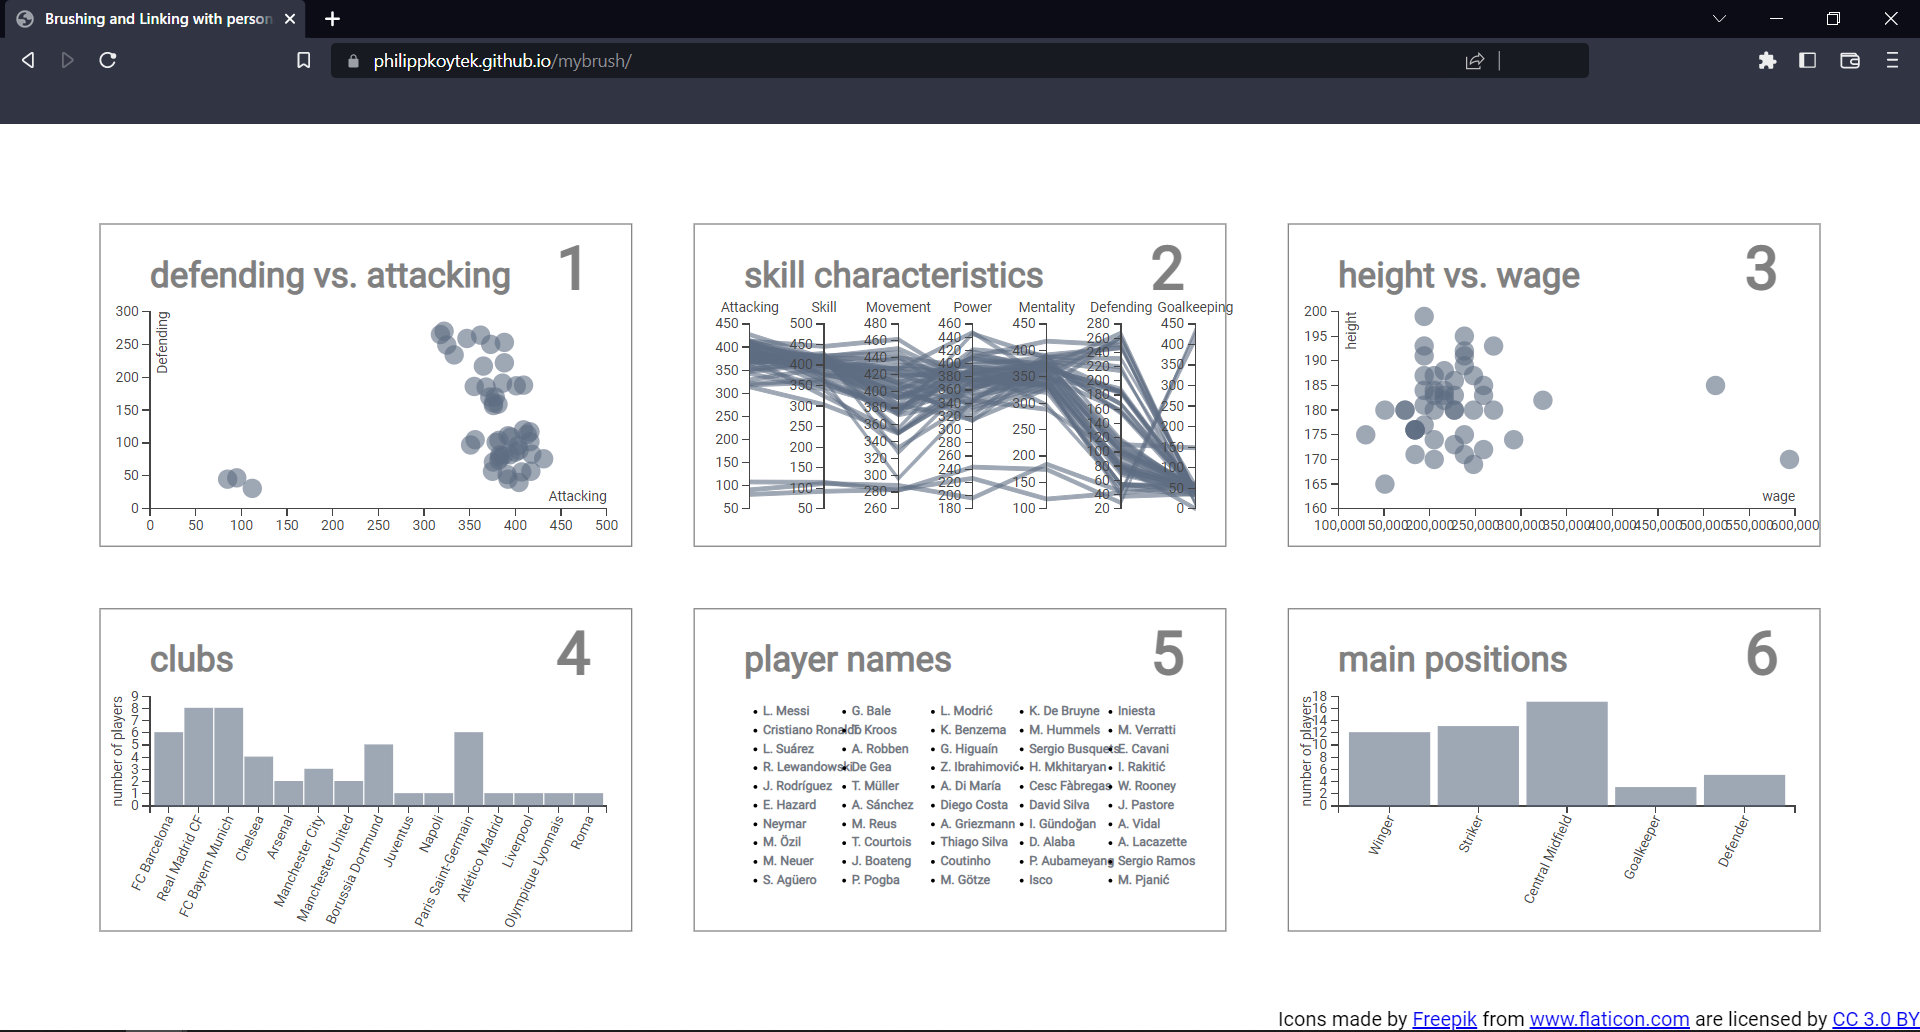
\includegraphics[keepaspectratio,width=\linewidth,height=\halfh, frame]
{images/screenshot-mybrush.png}

\caption[MyBrush Dashboard]
{%
MyBrush dashboard displaying the \emph{MyBrush Custom Football Players} dataset.
}
\label{fig:ScreenshotMyBrush}
\end{figure}




\section{XDAT}

XDAT \parencite{XDAT} is a multidimensional data analysis tool designed to
help users quickly and easily extract valuable insights from large,
complex data sets with many variables. XDAT is written in Java and is
available as a free software with the last update issued on
\yearmonthday{2020}{8}{26}. XDAT is available for Windows, macOS, and
Linux.

XDAT can visualize custom datasets and displays data in separate views.
XDAT displays the data with the following views: \emph{Parallel
Coordinates}, \emph{Table View} and \emph{Scatter Plot}. All of the
visualizations are interconnected through standard brushing and linking,
so that any changes or selections made in one view are reflected in all of
the other views. Figure~\ref{fig:ScreenshotXDAT} shows a screenshot of the
XDAT tool.




\begin{figure}[tp]
\centering
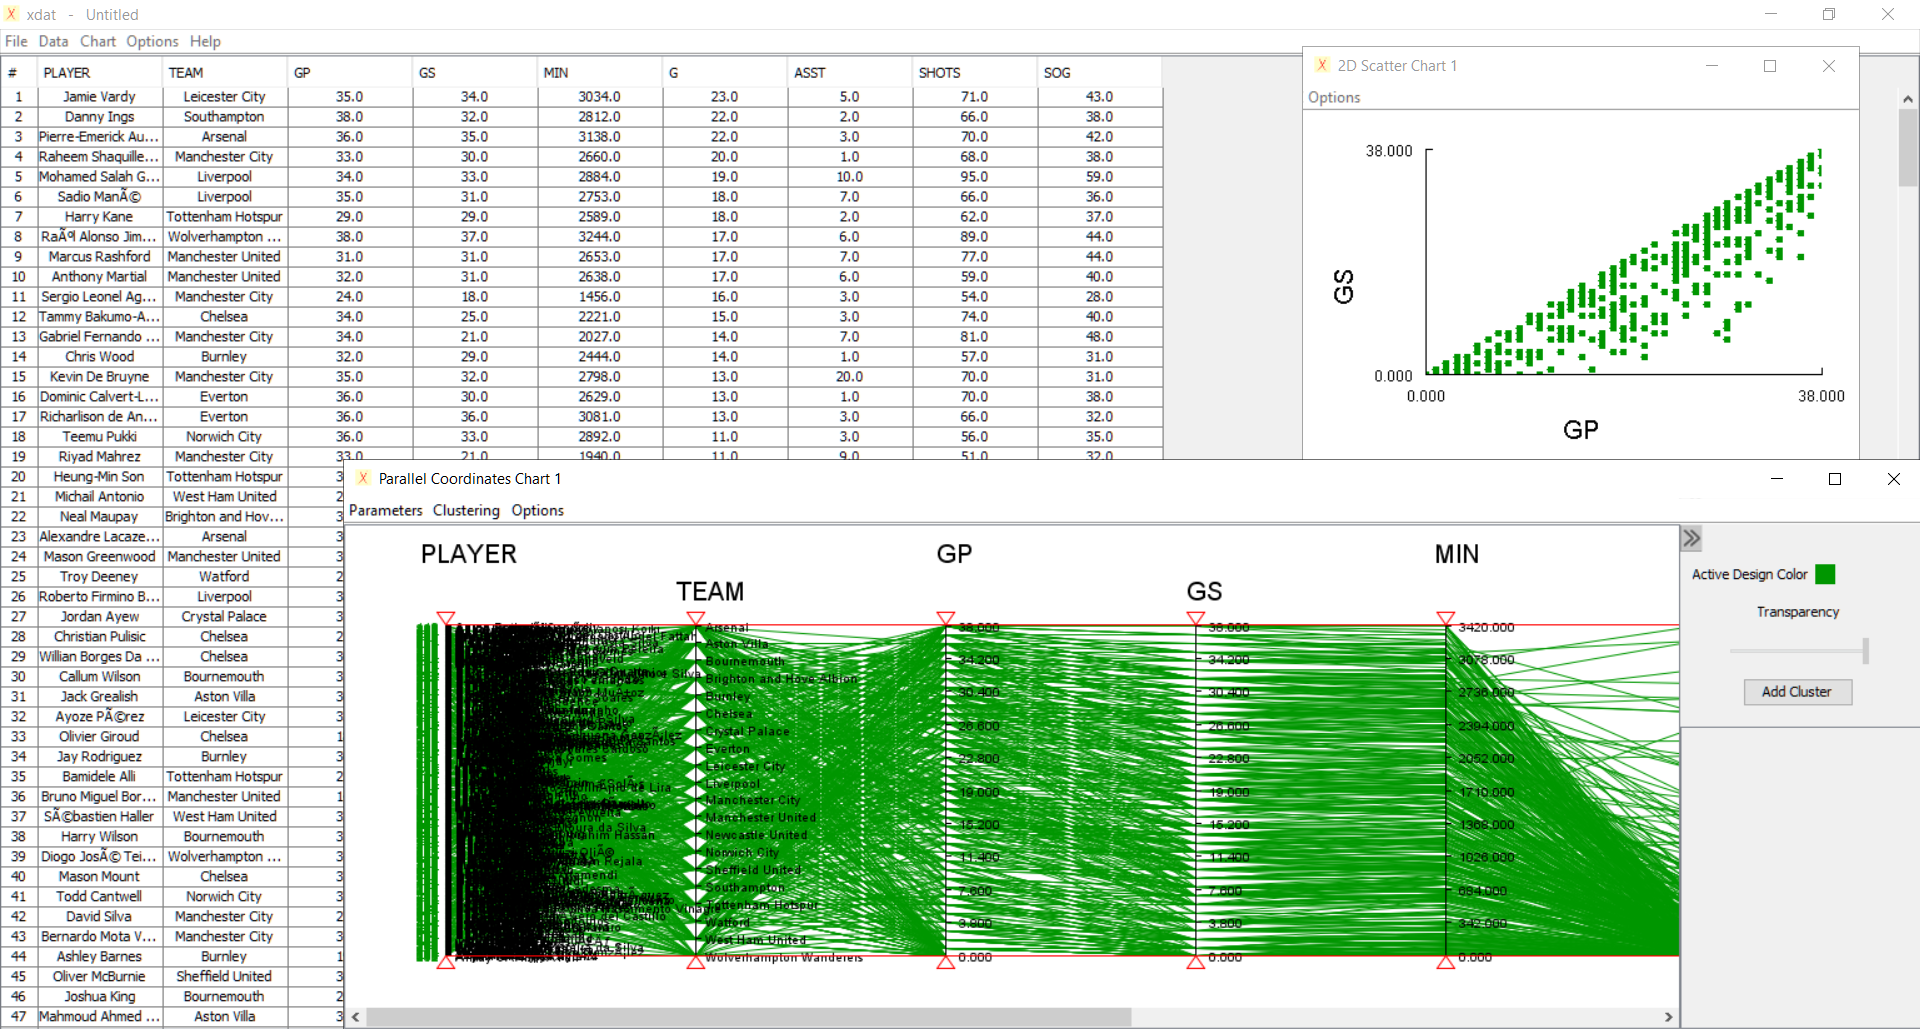
\includegraphics[keepaspectratio,width=\linewidth,height=\halfh]
{images/screenshot-xdat.png}

\caption[XDAT Dashboard]
{%
XDAT dashboard displaying the \emph{Premier League Player Stats} dataset.
}
\label{fig:ScreenshotXDAT}
\end{figure}



\section{TabuVis}

TabuVis \parencite{nguyen2013tabuvis} is a flexible and customizable
visual analytics system that is optimized for analyzing multidimensional
data. Its visualizations can be customized by domain experts to suit the
specific needs of the data being analyzed. TabuVis is written in Java and
is available as a free software with the latest update issued on
\yearmonthday{2022}{2}{19}. TabuVis is available for Windows, macOS, and
Linux.

TabuVis can visualize custom datasets and displays data in separate views.
TabuVis includes various features for analyzing data, such as the ability
to process data, add automatic marks, create custom interactive
visualizations, and filter the data. These features are designed to
support the entire data analysis process. TabuVis displays the data in the
following views: \emph{Scatter Plots}, \emph{Parallel Coordinates}, and
\emph{Star Plot}. TabuVis does not support brushing and linking.
Figure~\ref{fig:ScreenshotTabuVis} shows a screenshot of the TabuVis tool.




\begin{figure}[tp]
\centering
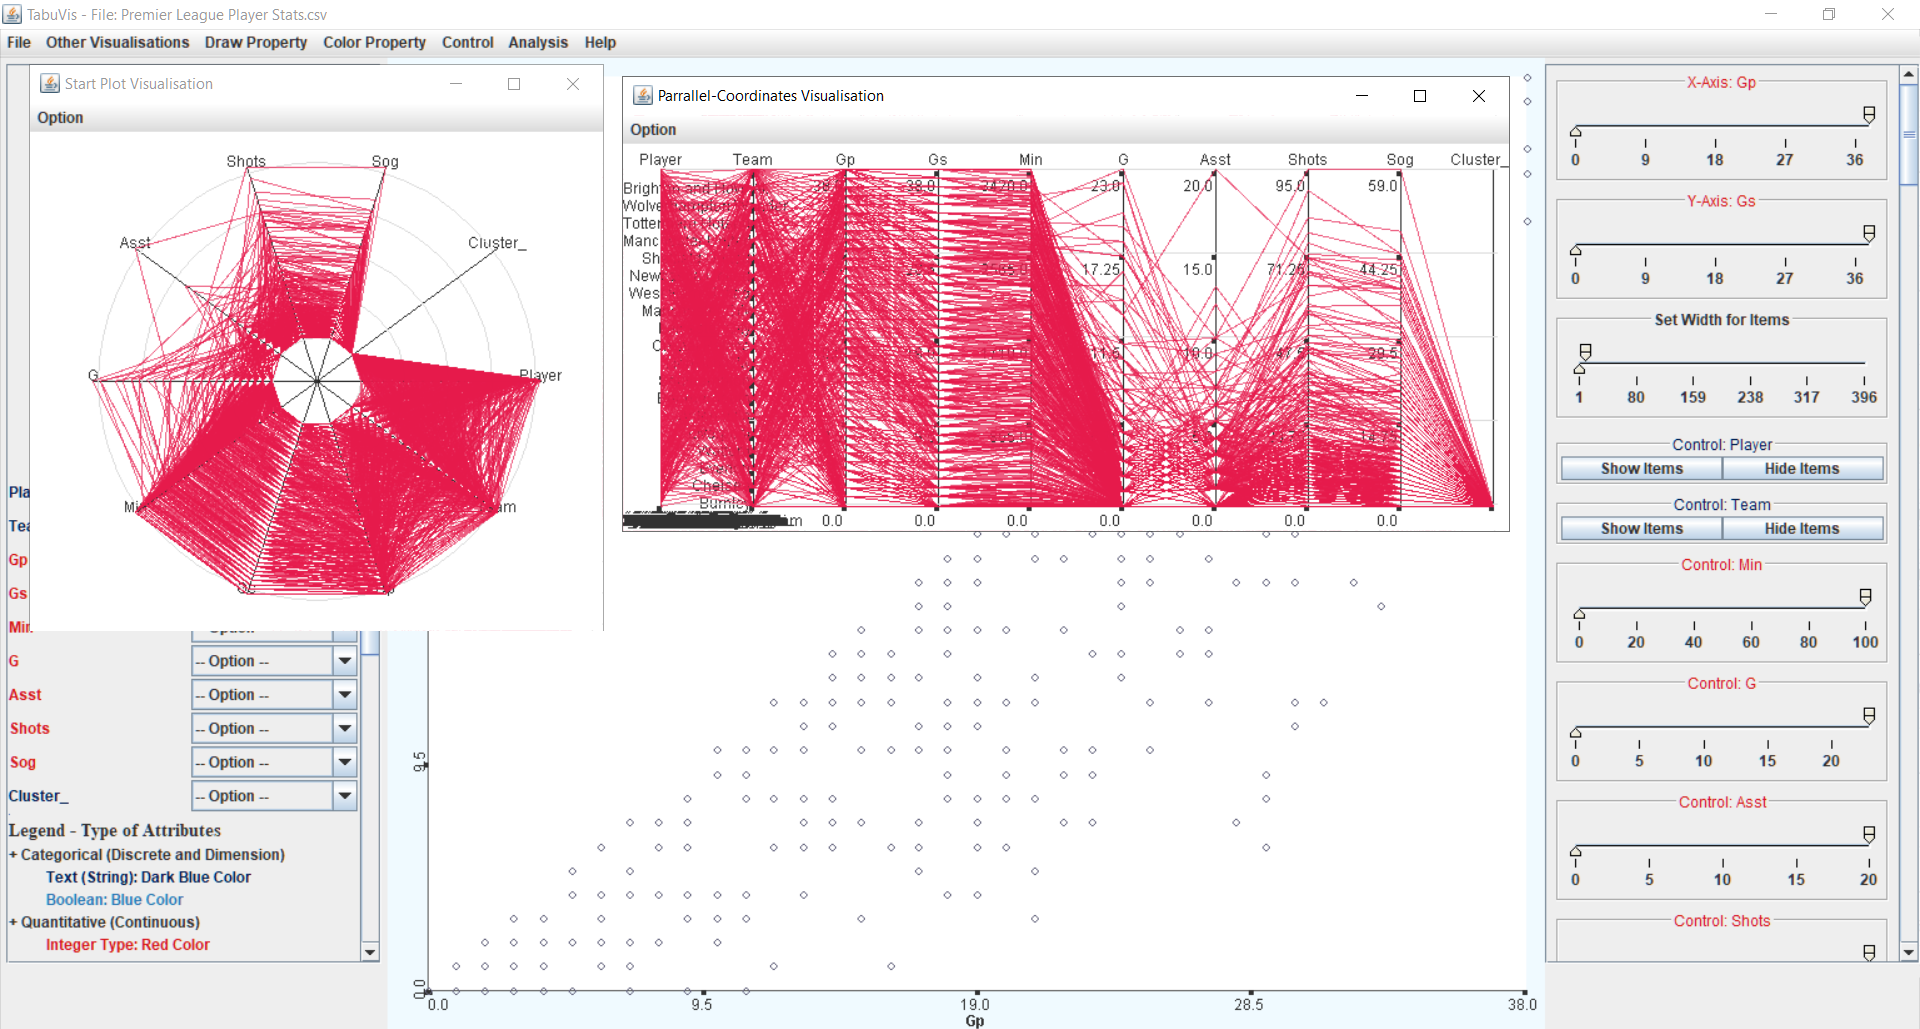
\includegraphics[keepaspectratio,width=\linewidth,height=\halfh]
{images/screenshot-tabuvis.png}

\caption[TabuVis Dashboard]
{%
TabuVis dashboard displaying the \emph{Premier League Player Stats} dataset.
}
\label{fig:ScreenshotTabuVis}
\end{figure}



\section{Parallax}

Parallax \parencite{inselberg2008parallel} is a tool for effectively analyzing
multidimensional datasets and discovering patterns, properties, and
relations in data. Parallax is written in \emph{x} and is available as
a commercial, closed-source with the latest update issued on \emph{x}.

Parallax can visualize custom datasets in a custom format. The format is a
simple text file with \emph{.dat} extension. The main part of Parallax
tool is a powerful parallel coordinates view, which enables queries. The
results of queries can be grouped and then shows seperately or in
combination with other queries. Parallax displays the data in the
following views: \emph{Scatter Plots}, \emph{Parallel Coordinates}, and
\emph{Distributions}. Parallax does not suport brushing and linking.
Figure~\ref{fig:ScreenshotParallax} shows a screenshot of the Parallax tool.




\begin{figure}[tp]
\centering
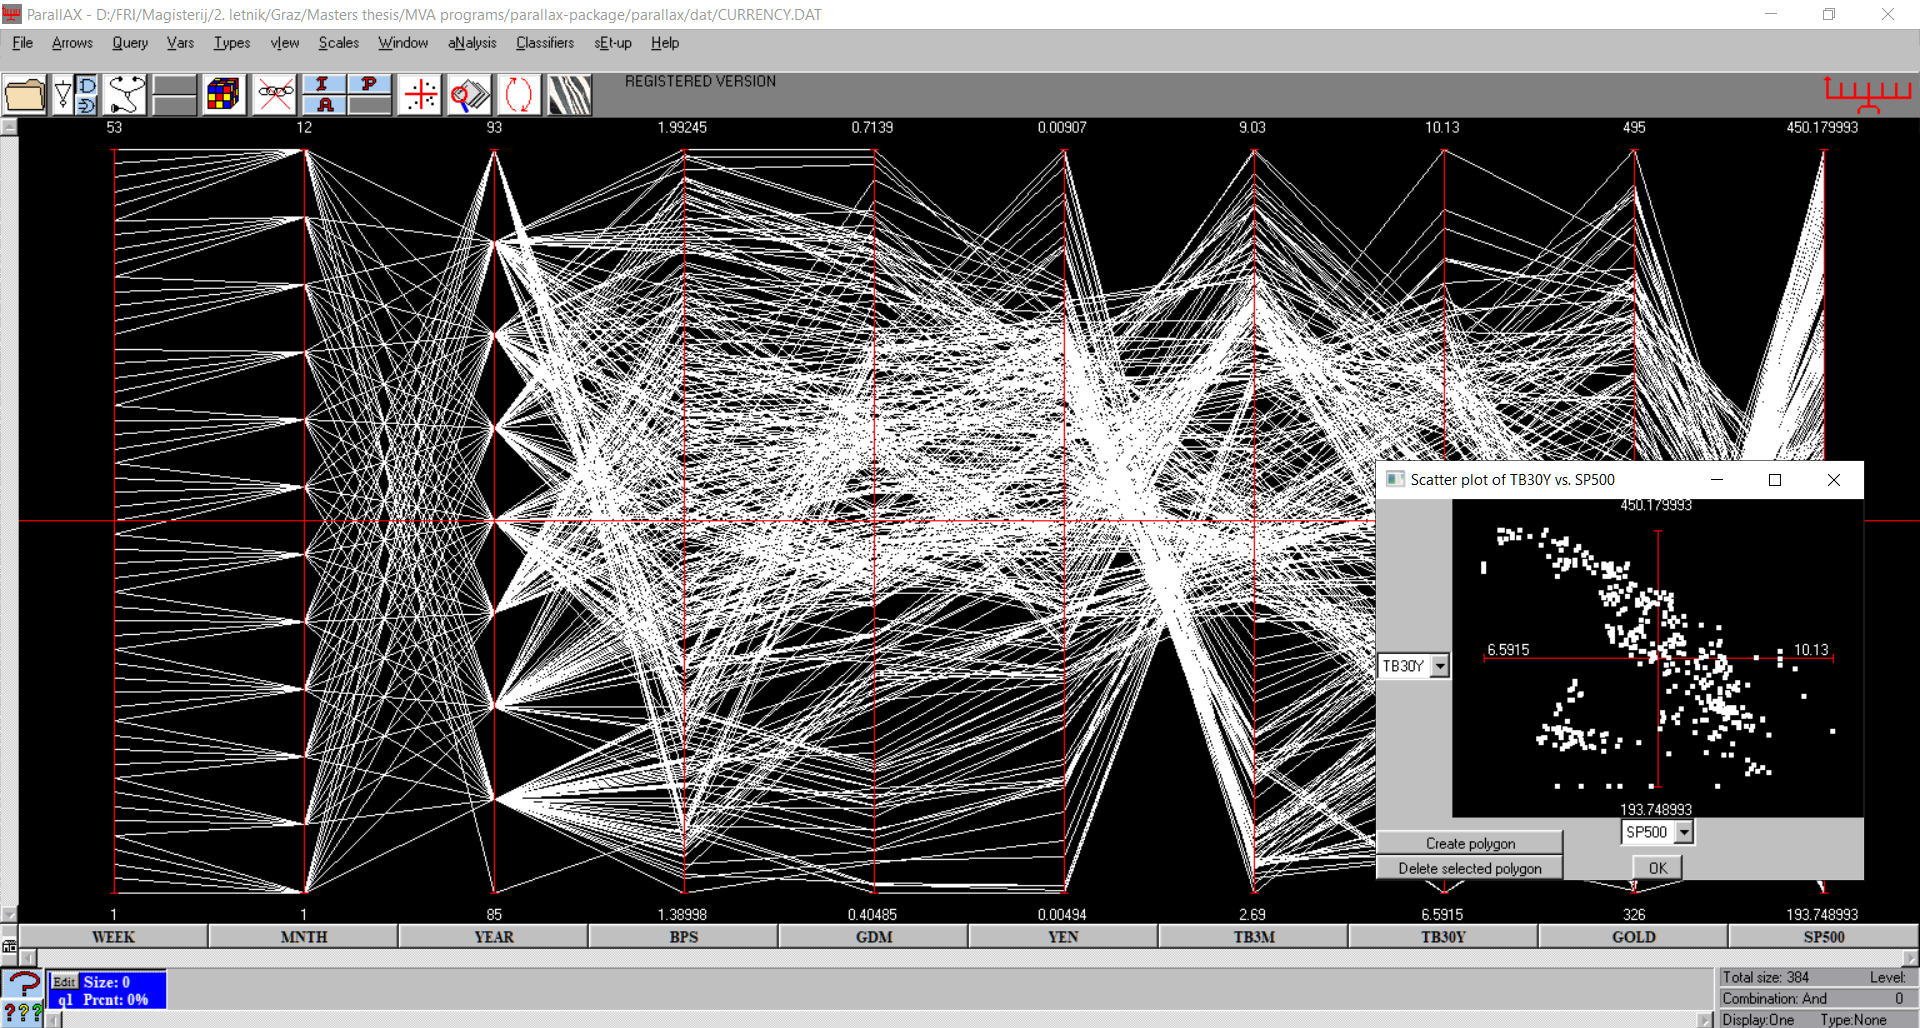
\includegraphics[keepaspectratio,width=\linewidth,height=\halfh]
{images/screenshot-parallax.png}

\caption[Parallax Dashboard]
{%
Parallax dashboard displaying a \emph{custom .dat} dataset.
}
\label{fig:ScreenshotParallax}
\end{figure}




\section{Comparison of Tools}

A comparison of general information of MVA software can be seen in
Table~\ref{tab:ToolsGeneral}. A comparison of features of MVA software can
be seen in Table~\ref{tab:ToolsFeatures}.




\begin{table}[tp]
\begin{scriptsize}
\tablestretch
\rowcolors{2}{}{tablerowcolour}
\centering
\begin{tabularx}{\linewidth}
{>{\kern-\tabcolsep}lXXXXXXXXX<{\kern-\tabcolsep}}
\toprule
~ & \textbf{InfoScope} & \textbf{High-D} & \textbf{GGobi} & \textbf{mVis}
& \textbf{Improvise} & \textbf{MyBrush} & \textbf{XDAT} & \textbf{TabuVis} & \textbf{Parallax}
\\
\midrule
%
Last Update: & \yearmonth{2007}{2} & \yearmonth{2022}{12} &
\yearmonth{2012}{6} & \yearmonth{2021}{1} & \yearmonth{2020}{10} &
\yearmonth{2017}{9} & \yearmonth{2020}{8} & \yearmonth{2022}{2} & ? \\
%
Licence: & Free demo & Commercial & Free, open-source & Free, open-source
& Free, open-source & Free, open-source & Free & Free & Commercial \\
%
Systems: & Win, Mac\-OS, Linux & Win, Mac\-OS, Linux & Win, Mac\-OS, Linux
& Win, Mac\-OS, Linux & Win, Mac\-OS, Linux & Web Browser & Win, Mac\-OS,
Linux & Win, Mac\-OS, Linux & Win, Mac\-OS, Linux \\
%
Language & ? & ? & C & Java & Java & JavaScript & Java & Java & ? \\
%
Installation: & Local & Local & Local & Local & Local & Online & Local &
Local & Local \\
%
\bottomrule
\end{tabularx}
\end{scriptsize}

\caption[Overview of MVA Tools]
{%
Overview of MVA tools.
}
\label{tab:ToolsGeneral}
\end{table}





\begin{table}[tp]
\begin{scriptsize}
\tablestretch
\rowcolors{2}{}{tablerowcolour}
\centering
\begin{tabularx}{\linewidth}
{>{\kern-\tabcolsep}lCCCCCCCCC<{\kern-\tabcolsep}}
\toprule
~ & \textbf{InfoScope} & \textbf{High-D} & \textbf{GGobi} & \textbf{mVis}
& \textbf{Improvise} & \textbf{MyBrush} & \textbf{XDAT} & \textbf{TabuVis}
& \textbf{Parallax} \\
\midrule
%
Custom Datasets: & & \checkmark & \checkmark & \checkmark & \checkmark & &
\checkmark & \checkmark & \checkmark \\
%
Brushing: & \checkmark & \checkmark & \checkmark & \checkmark & & \checkmark &
\checkmark & & \\
%
Linking: & \checkmark & \checkmark & \checkmark & \checkmark & & \checkmark &
\checkmark & & \\
%
Manual Grouping: & \checkmark & \checkmark & & \checkmark & & & \checkmark
& \checkmark & \checkmark \\
%
Automated Clustering: & & \checkmark & & \checkmark & & & & \checkmark & \checkmark \\
%
Table View: & \checkmark & \checkmark & & & \checkmark & & \checkmark & & \\
%
Scattter Plot: & & \checkmark & \checkmark & \checkmark & \checkmark &
\checkmark & \checkmark & \checkmark & \checkmark \\
%
Scatter Plot Matrix: & & \checkmark & \checkmark & \checkmark & \checkmark
& & & & \\
%
Parallel Coordinates: & \checkmark & \checkmark & \checkmark & \checkmark
& & \checkmark & \checkmark & \checkmark & \checkmark \\
%
Parallel Coordinates Matrix: & & \checkmark & & & & & & & \\
%
Similarity Map: & \checkmark & \checkmark & & \checkmark & \checkmark & &
& \checkmark & \\
%
Time Series: & & & \checkmark & & \checkmark & & & & \\
%
Distributions: & & \checkmark & \checkmark & & \checkmark & \checkmark & &
& \checkmark \\
%
Table Plot: & & \checkmark & & & \checkmark & & & & \\
%
Tree Map: & & \checkmark & & & \checkmark & & & & \\
%
Carto Plot: & \checkmark & \checkmark & & & \checkmark & & & & \\
%
\bottomrule
\end{tabularx}
\end{scriptsize}

\caption[Comparison of MVA Tools]
{%
Comparison of MVA tools.
}
\label{tab:ToolsFeatures}
\end{table}

